\documentclass{hipatia}
\usepackage{lipsum}
\usepackage{enumerate}
\usepackage{float}
%Use \DeclareMathOperator para definir novos
% operadores para o modo matemático
\DeclareMathOperator{\sen}{sen}

%Evite numerar teoremas
%Prefira nomeá-los
%Use os ambientes abaixo
\newtheorem*{theorem*}{Teorema}
\newtheorem*{lemma*}{Lema}
\newtheorem{problem*}{Problema}
\newtheorem*{solution*}{Solução}
% Evite títulos muito longos
\title{O Encontro na Cafeteria\\ e Outros Problemas}

\author{Yure Carneiro e Samuel Feitosa}
% Se for necessário diminuir a fonte do título 
% para caber no quadro, use
% \title{ \fontsize{28}{28}\selectfont Uma Nova Demonstração do\\  \fontsize{28}{28}\selectfont Teorema de Pitágoras}

% O Subtítulo é o nome da seção da revista
% Deve ser uma palavra de origem grega
\subtitle{Problema}
%\author{Hipátia de Alexandria e Carl F.  Gauss}
% A data não é necessária
%\date{October 2023}
% Não se preocupe com a numeração
% das páginas ou com o número da edição

%\newcommand{\sen}{\mathop{\rm sen}}
\newcommand{\tg}{\mathop{\rm tg}}
\newcommand{\cotg}{\mathop{\rm cotg}}
\newcommand{\cossec}{\mathop{\rm cossec}}
\newcommand{\mdc}{\mathop{\rm mdc}}
\newcommand{\arctg}{\mathop{\rm arctg}}
\newcommand{\A}{^{\circ}}
%\DeclarePairedDelimiter\abs{\lvert}{\rvert}

\begin{document}
\setcounter{page}{\problemapage}
\maketitle


\section{Soluções da Edição Anterior}

\begin{problem*}
Calcule o valor de $\int_0^{\pi/2} \frac{dx}{1 + (\tg x)^{2022}}$ é
\end{problem*}

\begin{solution*}
Seja 
\begin{eqnarray*}
I & = & \int_0^{\pi/2} \frac{dx}{1 + (\tg x)^{2022}} \\
  & = & \int_0^{\pi/2} \frac{(\cos x)^{2022} dx}{(\sen x)^{2022} + (\cos x)^{2022}}
\end{eqnarray*}

Com a mudança de variável $y=\pi/2-x$, temos $dy = -dx$ e

\begin{eqnarray*}
I & = &  \int_{\pi/2}^0 \frac{(\cos (\pi/2-y))^{2022} (-dy)}{(\sen (\pi/2-y))^{2022} + (\cos (\pi/2-y))^{2022}} \\
& = & \int_0^{\pi/2} \frac{(\sen y)^{2022} dy}{(\sen y)^{2022} + (\cos y)^{2022}}
\end{eqnarray*}
Portanto, 
$$I + I = \int_0^{\pi/2} \frac{(\sen x)^{2022}+(\cos x)^{2022} dx}{(\sen x)^{2022}+(\cos x)^{2022}} = \dfrac{\pi}{2}.$$
Assim, $I=\dfrac{\pi}{4}$.

\end{solution*}

\begin{problem*}
Encontre o valor de 

$$\displaystyle \int_0^{\pi/2} \cos^2 (\cos x)dx + \int_0^{\pi/2} \sen^2 (\sen x)dx .$$

\end{problem*}

\begin{solution*}
Com a mudança de variável $y=\pi/2-x$, temos $dy = -dx$ e 
\begin{eqnarray*}
\int_0^{\pi/2} \sen^2 (\sen x)dx & = & \int_{\pi/2}^{0} \sen^2 (\sen (\pi/2-y))(-dy) \\
                                & = & \int_{0}^{\pi/2} \sen^2 (\cos y)dy \\
\end{eqnarray*}
\noindent Como $\cos^2 (\cos x)+\sen^2(\cos x)=1$, segue que 
\begin{eqnarray*}
\int_0^{\pi/2} \cos^2 (\cos x)dx + \int_0^{\pi/2} \sen^2 (\sen x)dx & = & \\ 
\int_0^{\pi/2} \cos^2 (\cos x)dx + \int_0^{\pi/2} \sen^2 (\cos x)dx & = & \\
\int_0^{\pi/2} 1 dx & = & \pi/2
\end{eqnarray*}
\end{solution*}


\begin{problem*}
Seja $A_{2022} = (a_{ij})$ a matriz $2022 \times 2022$ definida por 

$$a_{ij} = \left \{ \begin{array}{cl} \sqrt{3}, & \text{se}\,\,i=j \\1, & \text{se}\,\,|i-j|=1 \\ 0 & \text{caso contrário} \end{array} \right .$$

\noindent Encontre o valor de  $\det A_{2022}$.

\end{problem*}

\begin{solution*}
Defina como $A_n$ uma matriz $n \times n $ definida pelas mesmas regras e seja $D_n = \det A_n$. Pelo desenvolimento do determinante pela regra de Laplace com relação a primeira linha, temos 
$$ D_n = \sqrt{3}D_{n-1}-D_{n-2}.$$
A equação característica é 

$$x^2-\sqrt{3}x+1=0,$$

\noindent que possui como raízes $\dfrac{\sqrt{3}\pm i}{2} = -iw$ ou $iw^2$. Aqui $w=\dfrac{-1+i\sqrt{3}}{2}$ é raíz cúbica da unidade, i.e, $w^3=1$. Resolvendo a recorrência, encontramos
$$D_n = \dfrac{(-iw)^{2n+2}-1}{(-iw)^n((-iw)^2-1)}$$
Daí, usando que $w^3=1$ e $w^2+w+1=0$, temos 
\begin{eqnarray*}
D_{2022} & = & \dfrac{(-iw)^{4046}-1}{(-iw)^{2022}((-iw)^2-1)} \\
         & = & \dfrac{-w^2-1}{-(-w^2-1)} \\
         & = & \dfrac{w}{-w} \\
         & = & -1.
\end{eqnarray*}
\end{solution*}


\begin{problem*}
Sejam $z = e^{\frac{2\pi i}{2023}} = \cos \frac{2\pi}{2023} + i\sen \frac{2\pi}{2023} $,
$$A = \{1, z, z^2, \ldots, z^{2022} \}$$
e
$$B = \{1, 1+z, 1+z+z^2, \ldots, 1+z+z^2+ \ldots+ z^{2022} \}.$$

\noindent Determine o número de elementos de $A \cap B$.
\end{problem*}

\begin{solution*}
Provaremos que $A \cap B = \{1\}$. Inicialmente, é claro que $1 \in A \cap B$. Por outro lado, veremos que não há outros elementos na interseção. Para isso, vamos mostrar que $|1 + z + z^2 + \ldots + z^n| \neq 1$ para todo $1 \le n \le 2022$. Veja que
\[
1 + z + z^2 + \ldots + z^n = \frac{z^{n+1}-1}{z-1}
\]
e, portanto,
\[
|1 + z + z^2 + \ldots + z^n| = \frac{|z^{n+1}-1|}{|z-1|}.
\]
Usando que $e^{i\theta}-1 = 2i \sen(\theta/2)e^{i\theta/2}$, segue que
\[
|1 + z + z^2 + \ldots + z^n| = \frac{\sin\left(\frac{(n+1)\pi}{2023}\right)}{\sin\left(\frac{\pi}{2023}\right)}.
\]
Para $1 \le n \le 2022$, temos que $\sen((n+1)\pi/2023) \ge 0$ e $\sen(\pi/2023) > 0$. Dessa forma, só poderíamos ter $|1 + z + z^2 + \ldots + z^n| = 1$ caso $\sen((n+1)\pi/2023) = \sen(\pi/2023)$, o que é impossível para $1 \le n \le 2022$.
\end{solution*}


\begin{problem*}
O famoso {\it Problema da Basileia}\footnote{Euler foi o primeiro a provar que $$\dfrac{\pi^2}{6} = \dfrac{1}{1^2}+\dfrac{1}{2^2}+\dfrac{1}{3^2}+\dfrac{1}{4^2}+\ldots .$$ Além dele, alguns membros da família Bernoulli, que também viviam na cidade da Basileia, tentaram obter esse resultado. Por conta disso esse resultado também ficou atrelado ao nome da cidade. } nos permite descobrir que 

$$\dfrac{\pi^2}{8} = \dfrac{1}{1^2}+\dfrac{1}{3^2}+\dfrac{1}{5^2}+\dfrac{1}{7^2}+\ldots .$$

\noindent Vamos usar a série anterior para encontrar a soma de outra série. Para cada $n \in \mathbb{N}$, defina como $a_n$ seu maior divisor positivo ímpar. Por exemplo, $a_{30} = 15$ e $a_{24}=3$. Encontre o valor da soma:

$$S = \dfrac{a_1}{1^3}+\dfrac{a_2}{2^3}+\dfrac{a_3}{3^3}+\ldots .$$
\end{problem*}

\begin{solution*}
Considere as séries geométricas

\begin{eqnarray*}
\dfrac{1}{1^3}+\dfrac{1}{(1\cdot 2)^3}+\dfrac{1}{(1\cdot 2^2)^3}+\dfrac{1}{(1\cdot 2^3)^3} + \ldots  & = & \dfrac{8}{7} \\
\dfrac{1}{1^3}+\dfrac{1}{(3\cdot 2)^3}+\dfrac{1}{(3\cdot 2^2)^3}+\dfrac{1}{(3\cdot 2^3)^3} + \ldots  & = & \dfrac{8}{7} \cdot \dfrac{1}{3^2} \\
\dfrac{1}{5^3}+\dfrac{1}{(5\cdot 2)^3}+\dfrac{1}{(5\cdot 2^2)^3}+\dfrac{1}{(5\cdot 2^3)^3} + \ldots  & = & \dfrac{8}{7} \cdot \dfrac{1}{5^2} \\  
\dfrac{1}{7^3}+\dfrac{1}{(7\cdot 2)^3}+\dfrac{1}{(7\cdot 2^2)^3}+\dfrac{1}{(7\cdot 2^3)^3} + \ldots  & = & \dfrac{8}{7} \cdot \dfrac{1}{7^2} \\
                  & \vdots & 
\end{eqnarray*}
Cada fração $\dfrac{a_n}{n^3}$ aparece exatamente uma vez em cada uma dessas séries. Portanto, a soma desejada é:

$$\dfrac{8}{7} \cdot \left ( \dfrac{1}{1^2}+ \dfrac{1}{3^2}+\dfrac{1}{5^2}+\dfrac{1}{7^2} + \ldots \right ) = \dfrac{8}{7} \cdot \dfrac{\pi^2}{8} =\dfrac{\pi^2}{7}.$$
\end{solution*}


\begin{problem*}
Bernardo está brincando de desenhar quadriláteros em um papel pontilhado como o da imagem a seguir. Os pontos pretos são vértices de quadradinhos de lado $1\,cm$ e os quadriláteros desenhados só podem usar como vértices os pontos pretos.


\begin{figure}[htbp]
\centering
		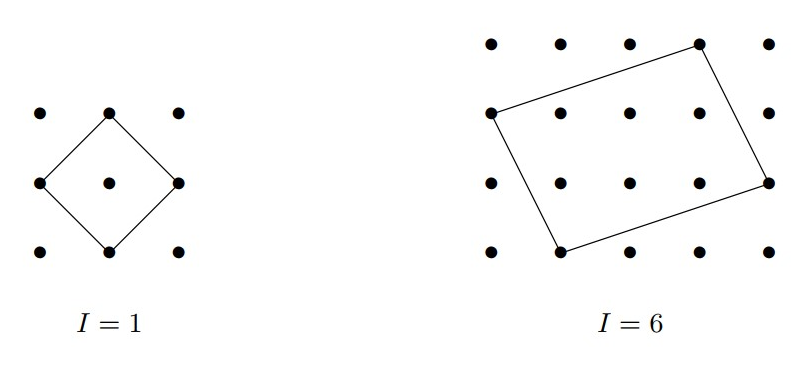
\includegraphics[scale=0.5]{F51.png}
\end{figure} 

\noindent A letra $I$ representa o número de pontos pretos no interior de cada quadrilátero.

\begin{enumerate}[a)]
%\item Dê exemplos de um losango e de uma pipa, cada um com $I=2$, no papel pontilhado \\

%\noindent Uma pipa é um quadrilátero em que as diagonais são perpendiculares e uma delas é dividida ao meio pela outra. Um losango é um exemplo de uma pipa.

\item Dê exemplos, por meio de um desenho, de quadrados com $I=4$ e $I=9$ no papel pontilhado.

%\item Dê um exemplo de um quadrado com $I=12$ no papel pontilhado.

\item Explique como Bernardo pode desenhar losangos contendo qualquer valor de pontos interiores desejado.

\item Qual é a menor área possível para um triângulo com vértices nos pontos do papel?
\end{enumerate}

\end{problem*}


\begin{solution*}
\begin{enumerate}[a)]
%\item Um exemplo de losango com $I=2$:

%\begin{figure}[htbp]
%	\centering
%		\includegraphics[scale=0.6]{F52.png}
%\end{figure} 

%\noindent Dois exemplos de pipas com $I=2$:

%\begin{figure}[htbp]
%	\centering%
%		\includegraphics[scale=0.6]{F53.png}
%\end{figure} 

\item Dois quadrados, um com $I=4$ e outro com $I=9$:

\begin{figure}[htbp]
	\centering
		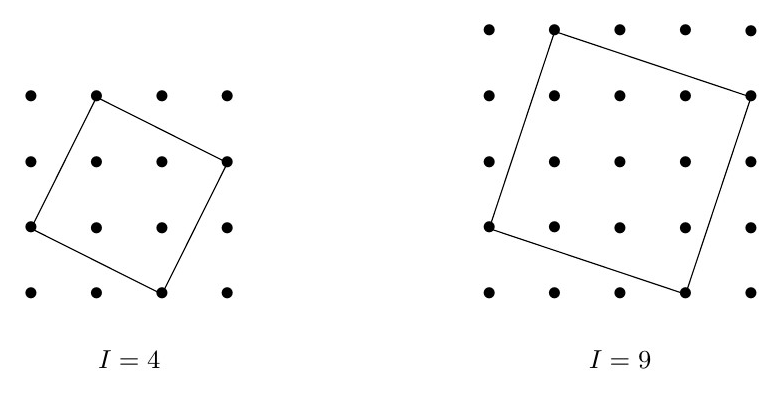
\includegraphics[scale=0.6]{F54.png}
\end{figure} 


%\item Um exemplo de quadrado com $I=12$:

%\begin{figure}[htbp]
%	\centering
%		\includegraphics[scale=0.6]{F55.png}
%\end{figure} 


\item Se $I$ é um número ímpar, podemos dispor $I+2$ pontos consecutivos na vertical e marcar como vértices do losango os extremos dessa sequência. Os outros dois vértices são os pontos nas verticais anterior e sucessora mais próximos do centro da sequência de pontos, como indicado nas figuras a seguir: 

\begin{figure}[htbp]
	\centering
		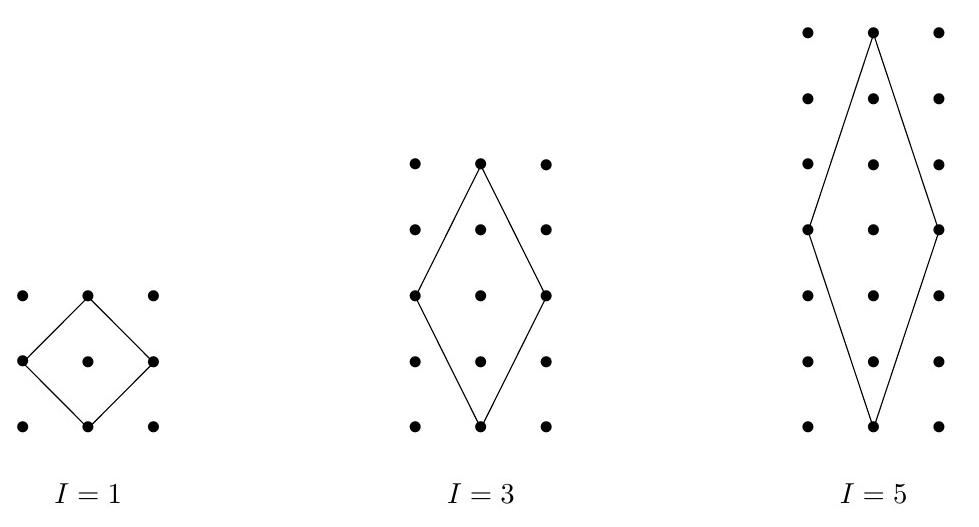
\includegraphics[scale=0.4]{F56.png}
\end{figure} 

\noindent Se $I$ é um número par, considere uma diagonal de $I+2$ pontos consecutivos formando $45^{\circ}$ com os lados do papel do reticulado. Os dois pontos extremos dessa diagonal serão vértices do losango. Os outros dois vértices são os $2$ pontos mais próximos do centro da diagonal, como indicado nas figuras a seguir: 

\begin{figure}[htbp]
	\centering
		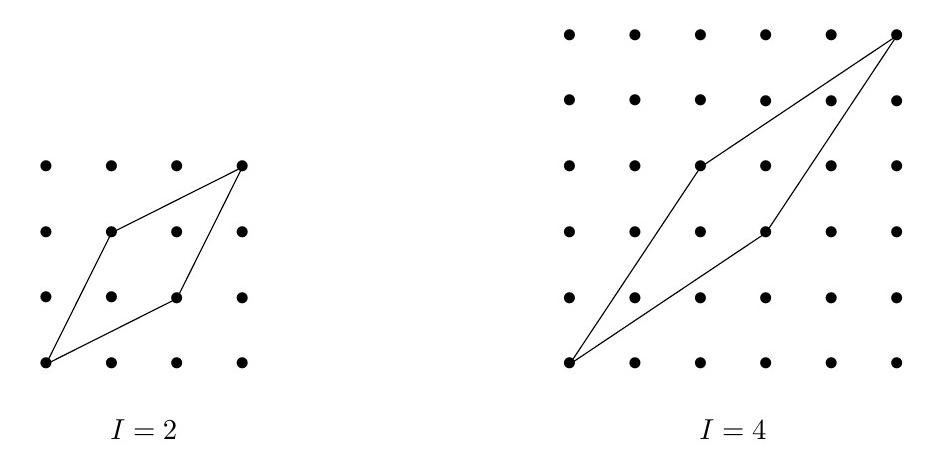
\includegraphics[scale=0.4]{F57.png}
\end{figure} 


\item Dado qualquer triângulo com vértices nos reticulados, se dois de seus vértices estão na horizontal ou vertical (em relação aos lados do papel), a distância entre eles é um número inteiro $b$. A altura $h$ do terceiro vértice a esses dois também é um inteiro $h$. A área do triângulo é, portanto, 

$$\dfrac{b \cdot h}{2} \geq \dfrac{1}{2}\,\mathrm{cm}^2$$

\noindent Veja que realmente existem triângulos com área $1/2$. Basta considerar um quadradinho $1 \times 1$ do papel e dividi-lo ao meio por uma de suas diagonais. Veja que o argumento anterior mostra que a área de qualquer triângulo com lados paralelos aos lados da folha é da forma $n/2$, em que $n$ é um número inteiro. Para terminar, precisamos considerar os triângulo $ABC$ que não possuem lados paralelos aos da folha, como na figura a seguir.


\begin{figure}[htbp]
	\centering
		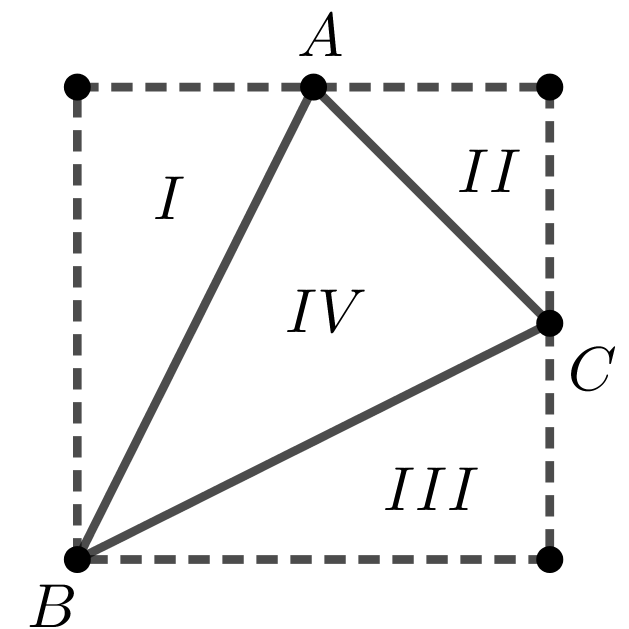
\includegraphics[scale=0.6]{F59.png}
\end{figure} 

\noindent Pelos seus vértices, trace retas paralelas aos lados das folhas. As interseções dessas retas são pontos dos reticulados, e, pelo argumento anterior, podemos garantir que as áreas das regiões $I$, $II$ e $III$ são números da forma $n/2$, com $n$ inteiro. Como a área de um retângulo com lados paralelos aos lados do tabuleiro é um número inteiro, contabilizando a diferença das áreas dos demais triângulos, podemos concluir que a área do triângulo $IV$ ou será um número inteiro ou metade de inteiro. Em qualquer caso, o seu valor mínimo é pelo menos $1/2$. 

\end{enumerate}

\noindent {\it Observação:} O Teorema de Pick permite calcular a área de qualquer polígono com vértices nos pontinhos da folha conhecendo o número de pontos interiores $I$ e o número de pontos no bordo da figura, que será chamado de $B$, através da fórmula:

$$A = I + \dfrac{B}{2}-1.$$

\begin{figure}[htbp]
	\centering
		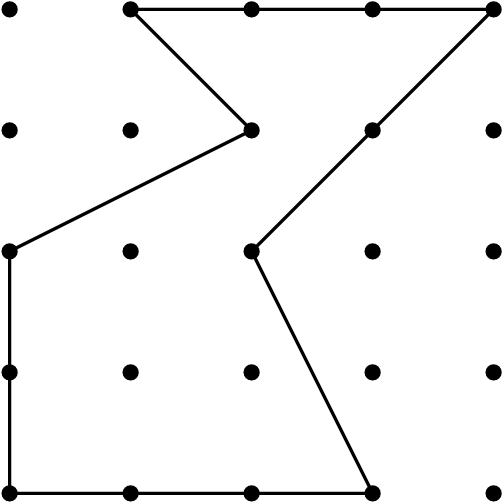
\includegraphics[scale=0.3]{F58.png}
\end{figure} 

\noindent Na figura anterior, $B=13$ e $I=3$, e assim a área do polígono é:

$$A = 3 + \dfrac{13}{2}-1 = 8,5\,cm^2.$$ 

\end{solution*}


\begin{problem*}
O número de todos os inteiros positivos de 64 dígitos sem zeros em sua representação e que são divisíveis por $101$ é par ou ímpar?
\end{problem*}

\begin{solution*}
	Precisamos criar alguma maneira de agrupar os números em pares. Seja $A = \underbrace{11 \ldots 11}_{64\,\,\, vezes}0$ repetições do número $1$. Como $1111$ é múltiplo de $101$ é fácil ver que  $A$ é múltiplo de $101$. Para todo número de $64$ dígitos $a=\overline{a_1a_2\ldots a_{63}a_{64}}$, sem zeros em sua representação decimal, considere o seu conjugado $b = \overline{b_1b_2\ldots b_{63}b_{64}} = (10-a_1)(10-a_2) \ldots (10-a_{64})$. Nenhum dígito de $a$ é igual a zero, portanto, cada número $10-a_i$ pertence ao conjunto $\{0,1,\ldots, 9\}$. Da equação $a+b=A$ obtemos que $a$ é divisível por $101$ se e somente se $b$ é divisível por $101$(lembre-se que $A$ é múltiplo de $101$). Como o único número que é igual ao seu conjugado é o número $\underbrace{55 \ldots 55}_{64\,\,\, vezes}$(que é múltiplo de $101$) e os demais números que satisfazem o enunciado podem ser pareados, concluímos que a quantidade procurada é ímpar.
\end{solution*}


\begin{problem*}
É possível arranjar os números $1,1,2,2,3,3, \ldots, 1986,1986$ em fila de modo que
entre quaisquer dois $i's$ hajam $(i-1)$ números? 
\end{problem*}


\begin{solution*}
Vamos tentar fazer alguns casos pequenos. É fácil ver que não conseguimos fazer o que o enunciado pede com os números $1,1,2,2$ mas com os números $1,1,2,2,3,3,4,4$ temos um exemplo:
$$
\begin{array}{cccccccc}
1^{\circ} & 2^{\circ} & 3^{\circ} & 4^{\circ} & 5^{\circ} & 6^{\circ} & 7^{\circ} & 8^{\circ} \\
a_3 & a_4 & a_2 & b_3 & b_2 & b_4 & a_1 & b_1 \\
{\bf 3}   & {\bf 4}   &  {\bf 2}  & {\bf 3}   & {\bf 2}   &  {\bf 4}  & {\bf 1}   & {\bf 1}
\end{array}
$$
Contando da esquerda para a direita, denotemos por $a_i$ e $b_i$ as posições do primeiro e segundo número $i$, respectivamente. No nosso exemplo, $a_2 = 3$ e $b_2 =5$. Como existem $i-1$ números entre dois números $i's$, devemos ter $b_i-a_i = i$. Se é possível escrever os números $1,1,2,2, \ldots n,n$ em linha como no enunciado, obtemos:

\begin{eqnarray*}
(a_1+a_2+ \ldots a_n) + (b_1+b_2+ \ldots + b_n)  & = &  \\
1 + 2 + \ldots + 2n  & = & n(2n+1)\\
(b_1 - a_1) + (b_2-a_2)+ \ldots (b_n-a_n) & = &  \\
1 + 2 + \ldots  + n & = & \dfrac{n(n+1)}{2}.
\end{eqnarray*} 

\noindent Somando as duas linhas,

\begin{eqnarray*}
2(b_1+b_2+ \ldots b_n) = \dfrac{n(5n+3)}{2}
\end{eqnarray*}

\noindent Como o lado esquerdo é sempre par, a fração $\dfrac{n(5n+3)}{2}$ deve ser um inteiro par. Isso já restringe os possíveis valores de $n$. Para $n=1986$,

\begin{eqnarray*}
\dfrac{n(5n+3)}{2} = 9863469
\end{eqnarray*}

\noindent é ímpar e consequentemente não é possível dispormos esses números em linha. Uma pergunta natural que você deve tentar descobrir é, para quais $n$, tal distribuição é possível. 
\end{solution*}


\begin{problem*}
Os alunos da $DMAT$ aprendem $n$ matérias no semestre. É verdade que para cada matéria exatamente 3 alunos são os melhores nessa matéria, e que para cada 2 matérias, existe exatamente um aluno que é um dos melhores nas duas.
Prove que:
\begin{enumerate}[a)]
\item Se $n=8$ existe um aluno que é um dos melhores em todas as matérias.
\item Se $n=7$, não é necessário que haja um aluno que é um dos melhores em todas as matérias. 
\end{enumerate}
\end{problem*}

\begin{solution*}
\begin{enumerate}[a)]
\item Vamos inicialmente mostrar que algum aluno deve ser o melhor em $4$ matérias. Suponha, por absurdo, que nenhum aluno é o melhor em $4$ materias. Seja $M_1$ uma matéria e $\{A,B,C\}$ os três alunos que são os melhores nessa matéria. Cada um deles pode estar em no máximo mais duas matérias e qualquer outra matéria deve ter um deles. Portanto, além de $M_1$, podem existir no máximo $2+2+2=6$ matérias. Isso é um absurdo, pois temos mais que $7$ matérias. Assim, existe algum aluno, que denotaremos por $P$, que é o melhor em $4$ matérias. Sejam $M_1, M_2, M_3$ e $M_4$ quatro matérias em que ele é o melhor. Vamos mostrar que $P$ é o melhor em todas as matérias. Suponha que $A$ não é um dos melhores alunos para a matéria $M$. Assim, cada um dos $3$ melhores alunos de $M$, devem estar nos $4$ conjuntos disjuntos: $M_1-\{P\}$, $M_2-\{P\}$, $M_3-\{P\}$ e $M_4-\{P\}$. Isso é um absurdo. Logo, $P$ é o melhor em todas as matérias. 
\item Para $n=7$, podemos produzir um exemplo usando o diagrama de Fano da figura a seguir. Cada ponto respresenta um aluno e cada reta assim como o círculo central representam as matérias. Note que cada matéria possa por $3$ pontos, que serão os melhores nela, e que quaisquer duas matérias possuem exatamente um ponto em comum.

\begin{figure}[H]
	\centering
		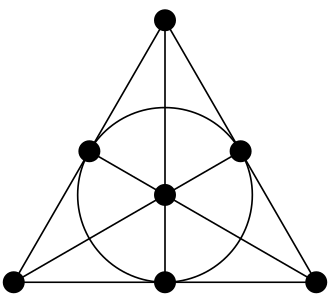
\includegraphics[scale=0.3]{fano.png}
\end{figure} 


\end{enumerate}
\end{solution*}


\section{Novos Problemas}


\section{Problemas Universitários}

\begin{problem*}
No plano complexo (plano de Argand-Gauss) um quadrato $ABCD$ tem centro no ponto $z=0$. 
    \begin{center}
       % \includegraphics[scale=0.6]%{ElonComplexos.png}

\begin{tikzpicture}[x=0.75pt,y=0.75pt,yscale=-0.6,xscale=0.6]
%uncomment if require: \path (0,300); %set diagram left start at 0, and has height of 300

%Shape: Axis 2D [id:dp4855606947862082] 
\draw [color={rgb, 255:red, 73; green, 135; blue, 206 }  ,draw opacity=1 ][line width=1.5]  (4.27,150.3) -- (324,150.3)(154.27,3) -- (154.27,258.3) (317,145.3) -- (324,150.3) -- (317,155.3) (149.27,10) -- (154.27,3) -- (159.27,10)  ;
%Straight Lines [id:da78389926760332] 
\draw [color={rgb, 255:red, 0; green, 0; blue, 0 }  ,draw opacity=1 ][line width=1.5]    (125.88,50.18) -- (54.82,175.88) ;
\draw [shift={(54.82,175.88)}, rotate = 119.48] [color={rgb, 255:red, 0; green, 0; blue, 0 }  ,draw opacity=1 ][fill={rgb, 255:red, 0; green, 0; blue, 0 }  ,fill opacity=1 ][line width=1.5]      (0, 0) circle [x radius= 4.36, y radius= 4.36]   ;
\draw [shift={(125.88,50.18)}, rotate = 119.48] [color={rgb, 255:red, 0; green, 0; blue, 0 }  ,draw opacity=1 ][fill={rgb, 255:red, 0; green, 0; blue, 0 }  ,fill opacity=1 ][line width=1.5]      (0, 0) circle [x radius= 4.36, y radius= 4.36]   ;
%Straight Lines [id:da528773304952439] 
\draw [color={rgb, 255:red, 0; green, 0; blue, 0 }  ,draw opacity=1 ][line width=1.5]    (180.52,246.95) -- (54.82,175.88) ;
\draw [shift={(54.82,175.88)}, rotate = 209.48] [color={rgb, 255:red, 0; green, 0; blue, 0 }  ,draw opacity=1 ][fill={rgb, 255:red, 0; green, 0; blue, 0 }  ,fill opacity=1 ][line width=1.5]      (0, 0) circle [x radius= 4.36, y radius= 4.36]   ;
\draw [shift={(180.52,246.95)}, rotate = 209.48] [color={rgb, 255:red, 0; green, 0; blue, 0 }  ,draw opacity=1 ][fill={rgb, 255:red, 0; green, 0; blue, 0 }  ,fill opacity=1 ][line width=1.5]      (0, 0) circle [x radius= 4.36, y radius= 4.36]   ;
%Straight Lines [id:da6921372221182511] 
\draw [color={rgb, 255:red, 0; green, 0; blue, 0 }  ,draw opacity=1 ][line width=1.5]    (251.58,121.24) -- (180.52,246.95) ;
\draw [shift={(180.52,246.95)}, rotate = 119.48] [color={rgb, 255:red, 0; green, 0; blue, 0 }  ,draw opacity=1 ][fill={rgb, 255:red, 0; green, 0; blue, 0 }  ,fill opacity=1 ][line width=1.5]      (0, 0) circle [x radius= 4.36, y radius= 4.36]   ;
\draw [shift={(251.58,121.24)}, rotate = 119.48] [color={rgb, 255:red, 0; green, 0; blue, 0 }  ,draw opacity=1 ][fill={rgb, 255:red, 0; green, 0; blue, 0 }  ,fill opacity=1 ][line width=1.5]      (0, 0) circle [x radius= 4.36, y radius= 4.36]   ;
%Shape: Square [id:dp25556747321772844] 
\draw  [color={rgb, 255:red, 0; green, 0; blue, 0 }  ,draw opacity=1 ][line width=1.5]  (125.88,50.18) -- (251.58,121.24) -- (180.52,246.95) -- (54.82,175.88) -- cycle ;

% Text Node
\draw (189.4,243.4) node [anchor=north west][inner sep=0.75pt]    {$A$};
% Text Node
\draw (258.4,104.4) node [anchor=north west][inner sep=0.75pt]    {$B$};
% Text Node
\draw (116.4,24.4) node [anchor=north west][inner sep=0.75pt]    {$C$};
% Text Node
\draw (40.4,188.4) node [anchor=north west][inner sep=0.75pt]    {$D$};


\end{tikzpicture}
\end{center}

\noindent Se o vértice $A$ encontra-se no afixo do número complexo $z_1$, determine o número complexo que representa o baricentro do triângulo $ABC$.
\end{problem*}

\begin{problem*}
Qual o número de pares ordenados $(a,b)$ de inteiros positivos $a, b$ tais que as seguintes condições sejam simultaneamente satisfeitas?

%M

\begin{itemize}
    \item [$(i)$]  
    $a\mid 6000$;
    \item [$(ii)$] 
    $1\le b \le \frac{6000}{a}$;
     \item [$(ii)$]
     $\operatorname{mdc}(a, b,\frac{6000}{a}) = 1$.
\end{itemize}
\end{problem*}

\begin{problem*}
Seja $r(x)$ o polinômio que é o resto na divisão de $x^{2050}$ por $x^5 + x^2  +1$.  Quantos coeficientes ímpares possui $r(x)$?
\end{problem*}

%\begin{problem*}
%A sequência $a_n$ é definida por $a_1=\sqrt{2}$ e, para $n \geq 1$, $a_{n+1}=\sqrt{2+a_n}$. %Determine
%$$\lim_{n \to \infty} 4^n(2-a_n).$$
%\end{problem*}

%\begin{problem*}
%Uma função $F: \mathbb{R} \rightarrow \mathbb{R}$ é contínua e $F(x) \cdot F(F(x))=1$ para %todo $x$ real. Sabendo que 
%$F(1000)=999$, encontre $F(500)$.
%Leningrado 188 página 20
%\end{problem*}

\begin{problem*}
Considere $\Gamma$ o lugar geométrico dos pontos $P$ do plano cuja razão entre a distância de $P$ à origem e a distância entre $P$ e a reta $y=-1$ é constante e igual a $\frac{1}{2}$. Qual a maior distância entre dois pontos de $\Gamma$?
	
\end{problem*}


\begin{problem*}
Seja $f : \mathbb{R} \rightarrow \mathbb{R}$ uma função ímpar e diferenciável satisfazendo:

\begin{itemize}
    \item $f(f(x)) = x$ para todo $x \in \mathbb{R}$;
    \item $f'(0) = 1$.
\end{itemize}

\noindent Mostre que $f(x) = -x$ para todo $x \in \mathbb{R}$.
	
\end{problem*}

\begin{problem*}
Sejam $A, B \in M_n(\mathbb{R})$. Prove que $\mbox{rank}(A) + \mbox{rank}(B) \leq n$ se, e somente se, existe uma matriz invertível $X \in M_n(\mathbb{R})$ tal que $AXB = O_n$, onde $O_n$ é a matriz nula de ordem $n$.
	
\end{problem*}

\section{Problemas de Matemática Elementar}

\begin{problem*}
Nas Olimpíadas de Pirajuba, existem $6$ competidores e $8$ dias de evento. Os três primeiros competidores de cada dia do evento recebem uma medalha, que pode ser de ouro, prata e bronze. Não existem empates e uma medalhade cada tipo é dada a apenas um atleta em cada dia do evento. Cada competidor recebe $5$ pontos por cada medalha de ouro, $3$ pontos por cada medalha de prata e $1$ ponto por cada medalha de bronze. Se Luciana, que é uma das competidoras, conseguiu um total de $27$ pontos no final do evento, qual o número máximo de medalhas de prata que ela pode ter recebido?
\end{problem*}

\begin{problem*}
Um encontro de britânicos e italianos em uma cafeteria reuniu 55 pessoas. Cada uma dessas pessoas pediu café ou chá. Sabemos que os britânicos sempre contam a verdade quando bebem chá e mentem quando bebem café. Já os italianos se comportam de modo oposto. Um repórter realizou uma rápida pesquisa e descobriu os seguintes fatos:
\begin{enumerate}
\item[1)] 44 pessoas responderam ``sim'' para a pergunta: ``Você está bebendo café?''
\item[2)] 33 pessoas responderam ``sim'' para a pergunta: ``Você é italiano?''
\item[3)] 22 pessoas concordaram com a afirmação: ``Está chovendo lá fora''.
\end{enumerate}

Quantos britânicos na cafeteria estavam tomando chá?
\end{problem*}

\begin{problem*}
Érica viajou para um país estrangeiro e sacou $\$800$ da moeda local em um banco. O caixa deu essa quantia usando notas de $\$20$, $\$50$ e $\$100$, usando pelo menos uma nota de cada tipo. De quantas maneiras diferentes ele pode ter feito esse pagamento para ela?
\end{problem*}

\begin{problem*}
Na malha a seguir, todos os quadradinhos possuem lados de mesma medida. Explique o porquê de os ângulos $\angle BAC$ e $\angle EDF$ possuírem a mesma medida. 
	
	\begin{center}	
		\begin{figure}[!h]
	\centering
	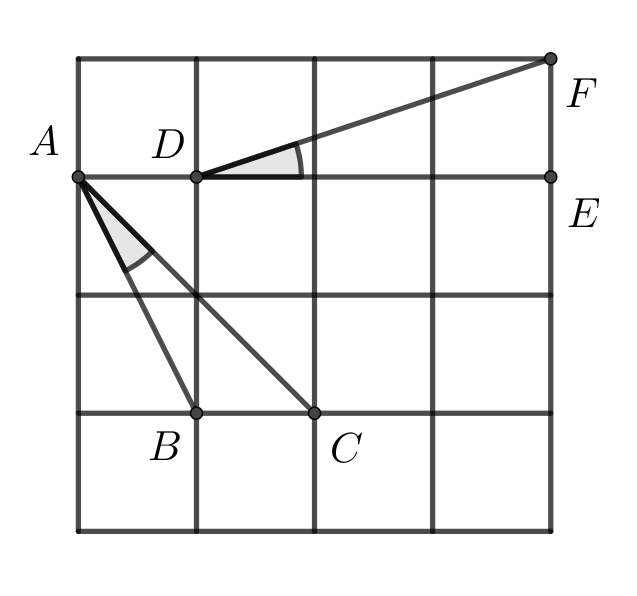
\includegraphics[width=0.3\linewidth]{2024S17.png}
\end{figure}
\end{center}	
\end{problem*}

\begin{problem*}
 Na figura a seguir, todos os triângulos são equiláteros e idênticos. Encontre a medida do ângulo $\angle ABC$.

\begin{center}


\tikzset{every picture/.style={line width=0.75pt}} %set default line width to 0.75pt        

\begin{tikzpicture}[x=0.75pt,y=0.75pt,yscale=-0.7,xscale=0.7]
%uncomment if require: \path (0,156); %set diagram left start at 0, and has height of 156

%Shape: Regular Polygon [id:dp42590613409471556] 
\draw   (101.6,127.59) -- (58.3,127.41) -- (80.11,90) -- cycle ;
%Shape: Regular Polygon [id:dp9891290054574801] 
\draw   (275.13,53.35) -- (231.83,53.16) -- (253.64,15.76) -- cycle ;
%Shape: Regular Polygon [id:dp432032311952501] 
\draw   (188.2,127.97) -- (144.9,127.78) -- (166.71,90.38) -- cycle ;
%Shape: Regular Polygon [id:dp965877053453182] 
\draw   (231.5,128.16) -- (188.2,127.97) -- (210.01,90.57) -- cycle ;
%Shape: Regular Polygon [id:dp60405412729036] 
\draw   (123.41,90.19) -- (80.11,90) -- (101.92,52.6) -- cycle ;
%Shape: Regular Polygon [id:dp38852321404456824] 
\draw   (166.71,90.38) -- (123.41,90.19) -- (145.22,52.78) -- cycle ;
%Shape: Regular Polygon [id:dp4093779740138518] 
\draw   (210.01,90.57) -- (166.71,90.38) -- (188.52,52.97) -- cycle ;
%Shape: Regular Polygon [id:dp2029637416434491] 
\draw   (80.11,90) -- (36.81,89.81) -- (58.62,52.41) -- cycle ;
%Shape: Regular Polygon [id:dp5343248854665051] 
\draw   (253.31,90.76) -- (210.01,90.57) -- (231.83,53.16) -- cycle ;
%Shape: Regular Polygon [id:dp6566631146501606] 
\draw   (101.92,52.6) -- (58.62,52.41) -- (80.44,15) -- cycle ;
%Shape: Regular Polygon [id:dp48167753179322537] 
\draw   (145.22,52.78) -- (101.92,52.6) -- (123.74,15.19) -- cycle ;
%Shape: Regular Polygon [id:dp6529080377153083] 
\draw   (188.52,52.97) -- (145.22,52.78) -- (167.04,15.38) -- cycle ;
%Shape: Regular Polygon [id:dp19072620498257065] 
\draw   (231.83,53.16) -- (188.52,52.97) -- (210.34,15.57) -- cycle ;
%Shape: Regular Polygon [id:dp5318721444025281] 
\draw   (144.9,127.78) -- (101.6,127.59) -- (123.41,90.19) -- cycle ;
%Shape: Regular Polygon [id:dp8872816823086344] 
\draw   (58.62,52.41) -- (15.32,52.22) -- (37.14,14.81) -- cycle ;
%Shape: Regular Polygon [id:dp3941974327848188] 
\draw   (37.27,14.73) -- (80.57,15.08) -- (58.62,52.41) -- cycle ;
%Shape: Regular Polygon [id:dp08330668174925715] 
\draw   (80.57,14.92) -- (123.87,15.27) -- (101.92,52.6) -- cycle ;
%Shape: Regular Polygon [id:dp1474450531110959] 
\draw   (123.87,15.27) -- (167.17,15.62) -- (145.22,52.94) -- cycle ;
%Shape: Regular Polygon [id:dp41036037730085884] 
\draw   (167.17,15.62) -- (210.47,15.97) -- (188.52,53.29) -- cycle ;
%Shape: Regular Polygon [id:dp6445074971855875] 
\draw   (210.47,15.97) -- (253.77,16.31) -- (231.82,53.64) -- cycle ;
%Shape: Regular Polygon [id:dp5435506141115087] 
\draw   (15.32,52.06) -- (58.62,52.41) -- (36.67,89.73) -- cycle ;
%Shape: Regular Polygon [id:dp045093785101125605] 
\draw   (36.81,89.81) -- (80.11,90.16) -- (58.16,127.48) -- cycle ;
%Shape: Regular Polygon [id:dp8659408226581283] 
\draw   (231.82,52.64) -- (275.12,52.99) -- (253.17,90.31) -- cycle ;
%Shape: Regular Polygon [id:dp00010682129482875169] 
\draw   (210.01,90.41) -- (253.31,90.76) -- (231.36,128.08) -- cycle ;
%Straight Lines [id:da8432136554916697] 
\draw [color={rgb, 255:red, 0; green, 0; blue, 0 }  ,draw opacity=1 ][line width=1.5]    (36.81,89.81) -- (231.36,128.08) ;
\draw [shift={(231.36,128.08)}, rotate = 11.13] [color={rgb, 255:red, 0; green, 0; blue, 0 }  ,draw opacity=1 ][fill={rgb, 255:red, 0; green, 0; blue, 0 }  ,fill opacity=1 ][line width=1.5]      (0, 0) circle [x radius= 4.36, y radius= 4.36]   ;
\draw [shift={(36.81,89.81)}, rotate = 11.13] [color={rgb, 255:red, 0; green, 0; blue, 0 }  ,draw opacity=1 ][fill={rgb, 255:red, 0; green, 0; blue, 0 }  ,fill opacity=1 ][line width=1.5]      (0, 0) circle [x radius= 4.36, y radius= 4.36]   ;
%Straight Lines [id:da36206940631647433] 
\draw [color={rgb, 255:red, 0; green, 0; blue, 0 }  ,draw opacity=1 ][line width=1.5]    (231.5,128.16) -- (253.77,16.31) ;
\draw [shift={(253.77,16.31)}, rotate = 281.26] [color={rgb, 255:red, 0; green, 0; blue, 0 }  ,draw opacity=1 ][fill={rgb, 255:red, 0; green, 0; blue, 0 }  ,fill opacity=1 ][line width=1.5]      (0, 0) circle [x radius= 4.36, y radius= 4.36]   ;
\draw [shift={(231.5,128.16)}, rotate = 281.26] [color={rgb, 255:red, 0; green, 0; blue, 0 }  ,draw opacity=1 ][fill={rgb, 255:red, 0; green, 0; blue, 0 }  ,fill opacity=1 ][line width=1.5]      (0, 0) circle [x radius= 4.36, y radius= 4.36]   ;

% Text Node
\draw (20,94.4) node [anchor=north west][inner sep=0.75pt]    {$A$};
% Text Node
\draw (233.5,131.56) node [anchor=north west][inner sep=0.75pt]    {$B$};
% Text Node
\draw (267,6.4) node [anchor=north west][inner sep=0.75pt]    {$C$};


\end{tikzpicture}

\end{center}
\end{problem*}

\begin{problem*}
Prove que $$\frac{1}{15} < \frac{1}{2}\cdot \frac{3}{4} \cdot \frac{5}{6} \cdots \frac{99}{100} < \frac{1}{12}$$
	
\end{problem*}

\begin{problem*}
Avalie a soma simplificando ao máximo sua expressão $$\frac{2}{0! + 1! + 2!} + \frac{3}{1! + 2! + 3!} + \cdots + \frac{2024}{2022! + 2023! + 2024!} $$
	
\end{problem*}

\nocite{*}
\vfill


\pagebreak 



\end{document}

% Mini bios 
% Seja informal e divertido
% Prefira fotos com fundo branco
\begin{wrapfigure}{L}{1.7cm}
	\centering
	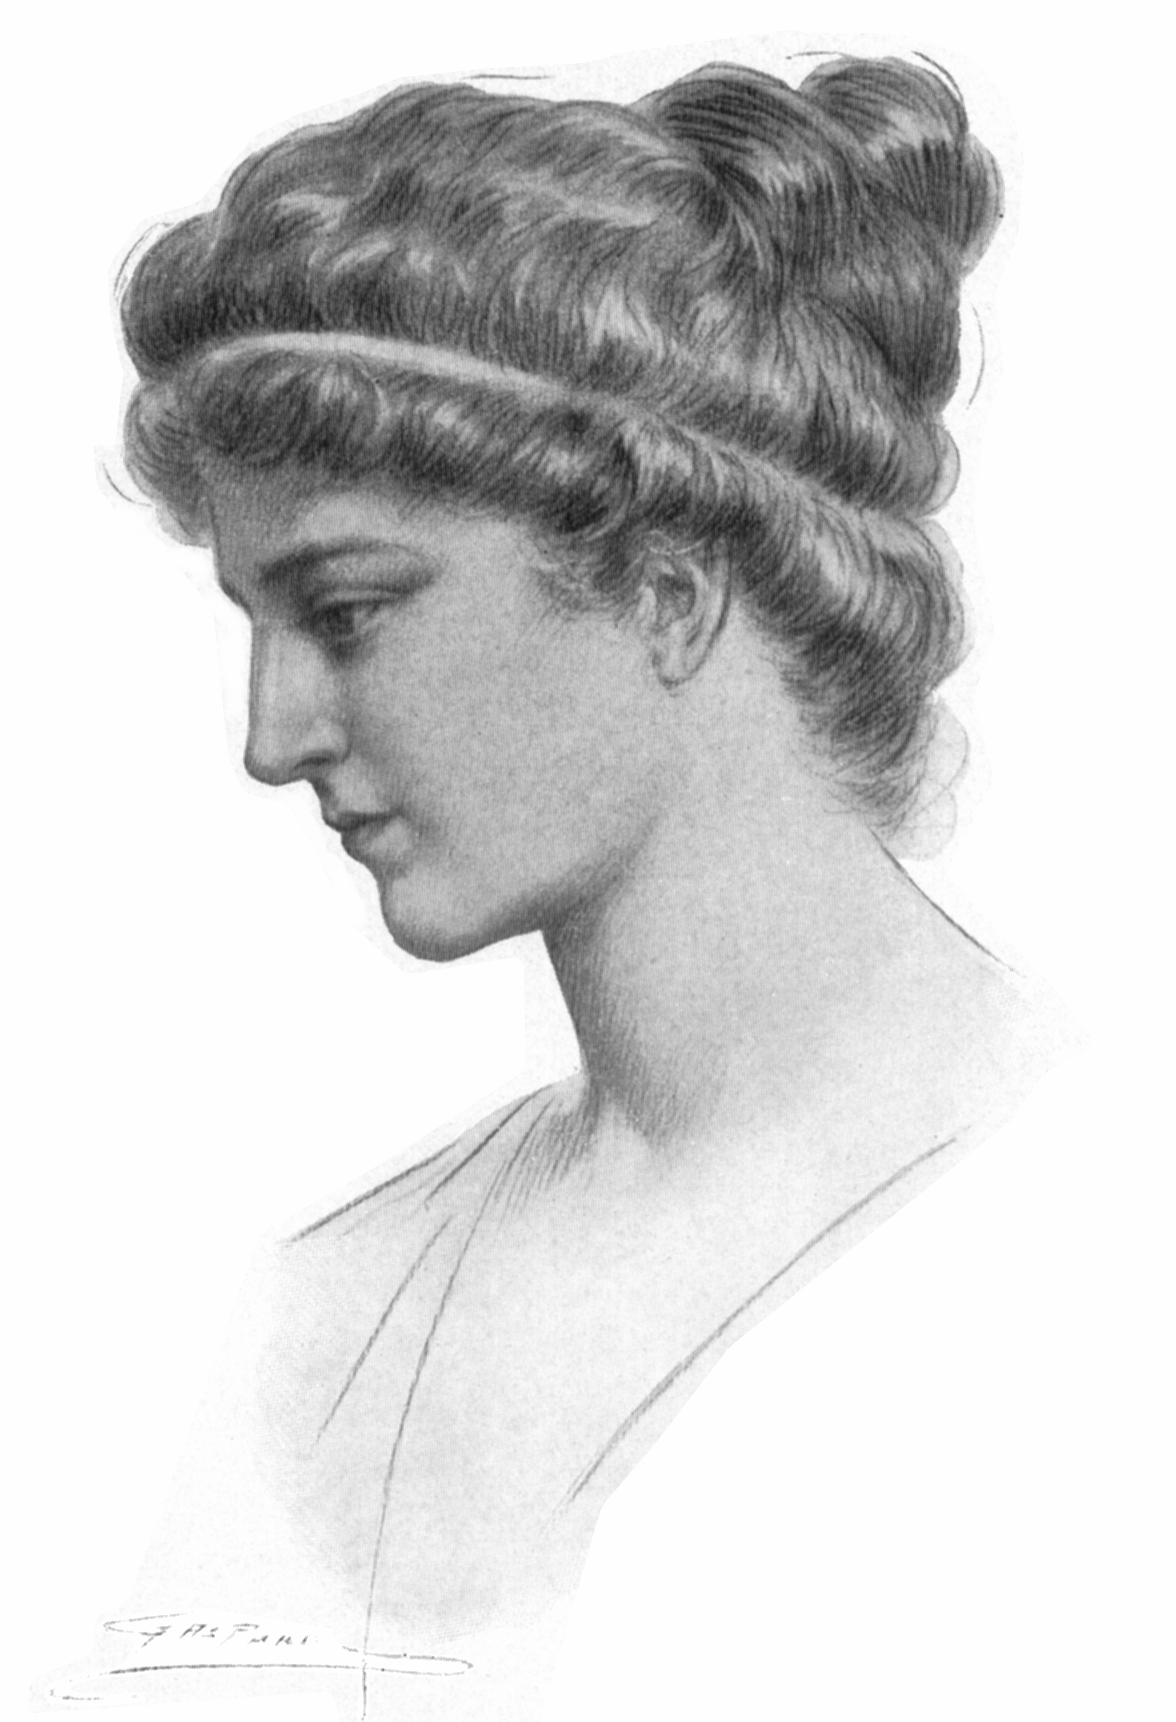
\includegraphics[width=2cm]{Hypatia_portrait.png}
\end{wrapfigure}\noindent
Hipátia de Alexandria é uma filósofa neoplatônica grega do Egito Romano. É a primeira mulher documentada como tendo sido matemática. Como chefe da escola platônica em Alexandria, também leciona filosofia e astronomia.

\vspace{1cm}
\begin{wrapfigure}{L}{1.7cm}
	\vspace{-10pt}
	\centering
	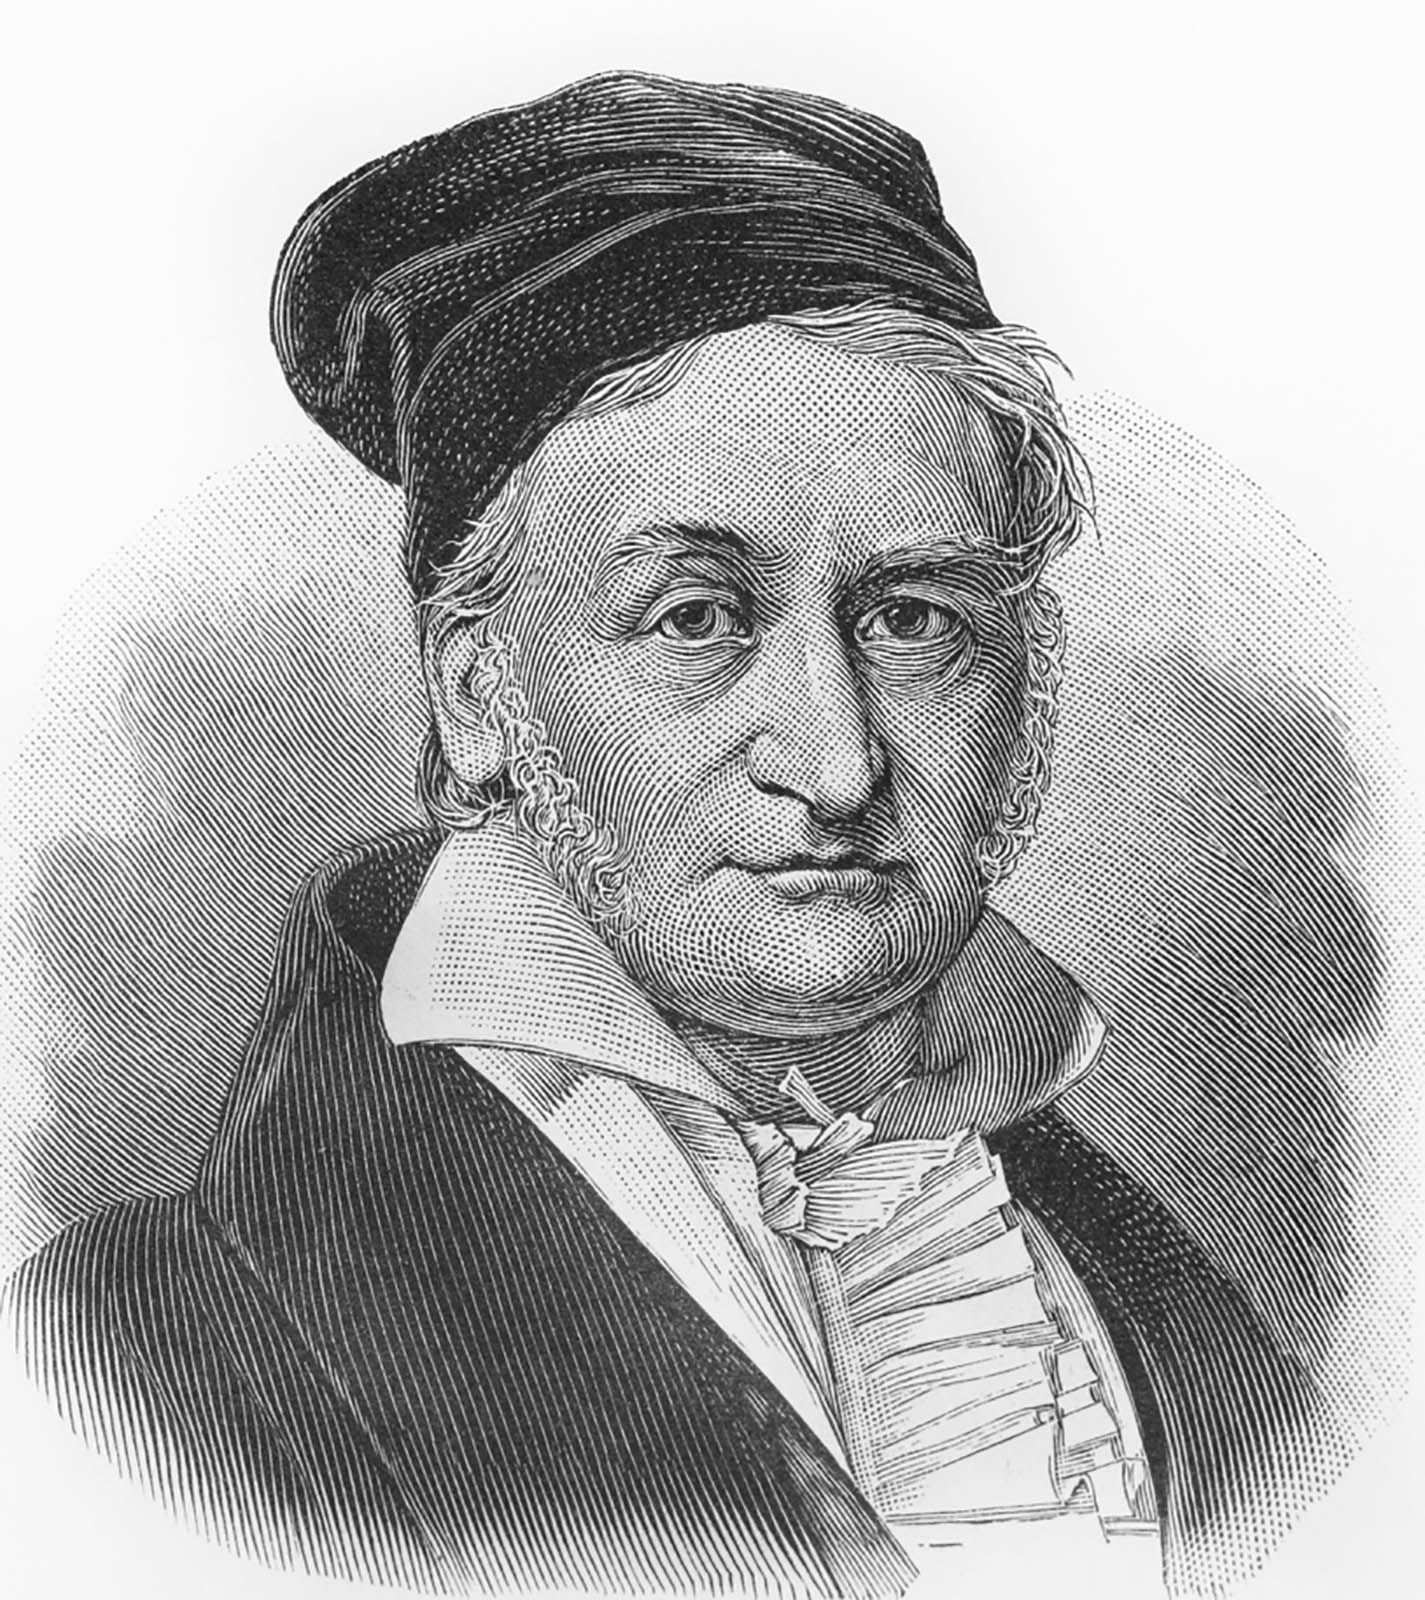
\includegraphics[width=2cm]{Carl-Friedrich-Gauss-engraving.jpg}
\end{wrapfigure}\noindent
Johann Carl Friedrich Gauss é um matemático, astrônomo e físico alemão que trabalha em diversas áreas da ciência, dentre elas a teoria dos números, estatística, análise matemática, geometria diferencial, geodésia, geofísica, eletroestática, astronomia e óptica.

Alguns se referem a ele como \emph{princeps mathematicorum} (em latim: ``o príncipe da matemática'' ou ``o mais notável dos matemáticos'').


\begin{figure}[htb!]
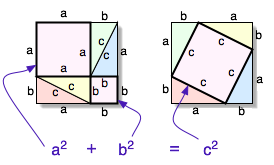
\includegraphics[width=8cm]{Pythagorean_proof.png}
\caption{Ideia geométrica da demonstração.}   
\end{figure}



